\section{Framework pour la modélisation des SdSs}

\begin{frame}{Concepts et objectifs de la modélisation d'un SdS}

\begin{block}{Objectifs }
\begin{itemize}
\item Exactitude : modéliser les CSs, leurs ressources et objectifs
d'interaction
\item Précision : modéliser les décisions architecturales 
\end{itemize}
\end{block}

\begin{block}{Problématique}
La frontière des SdSs est floue. Il est difficile de savoir quelles
informations ont un impact sur le SdS.\\
\centering
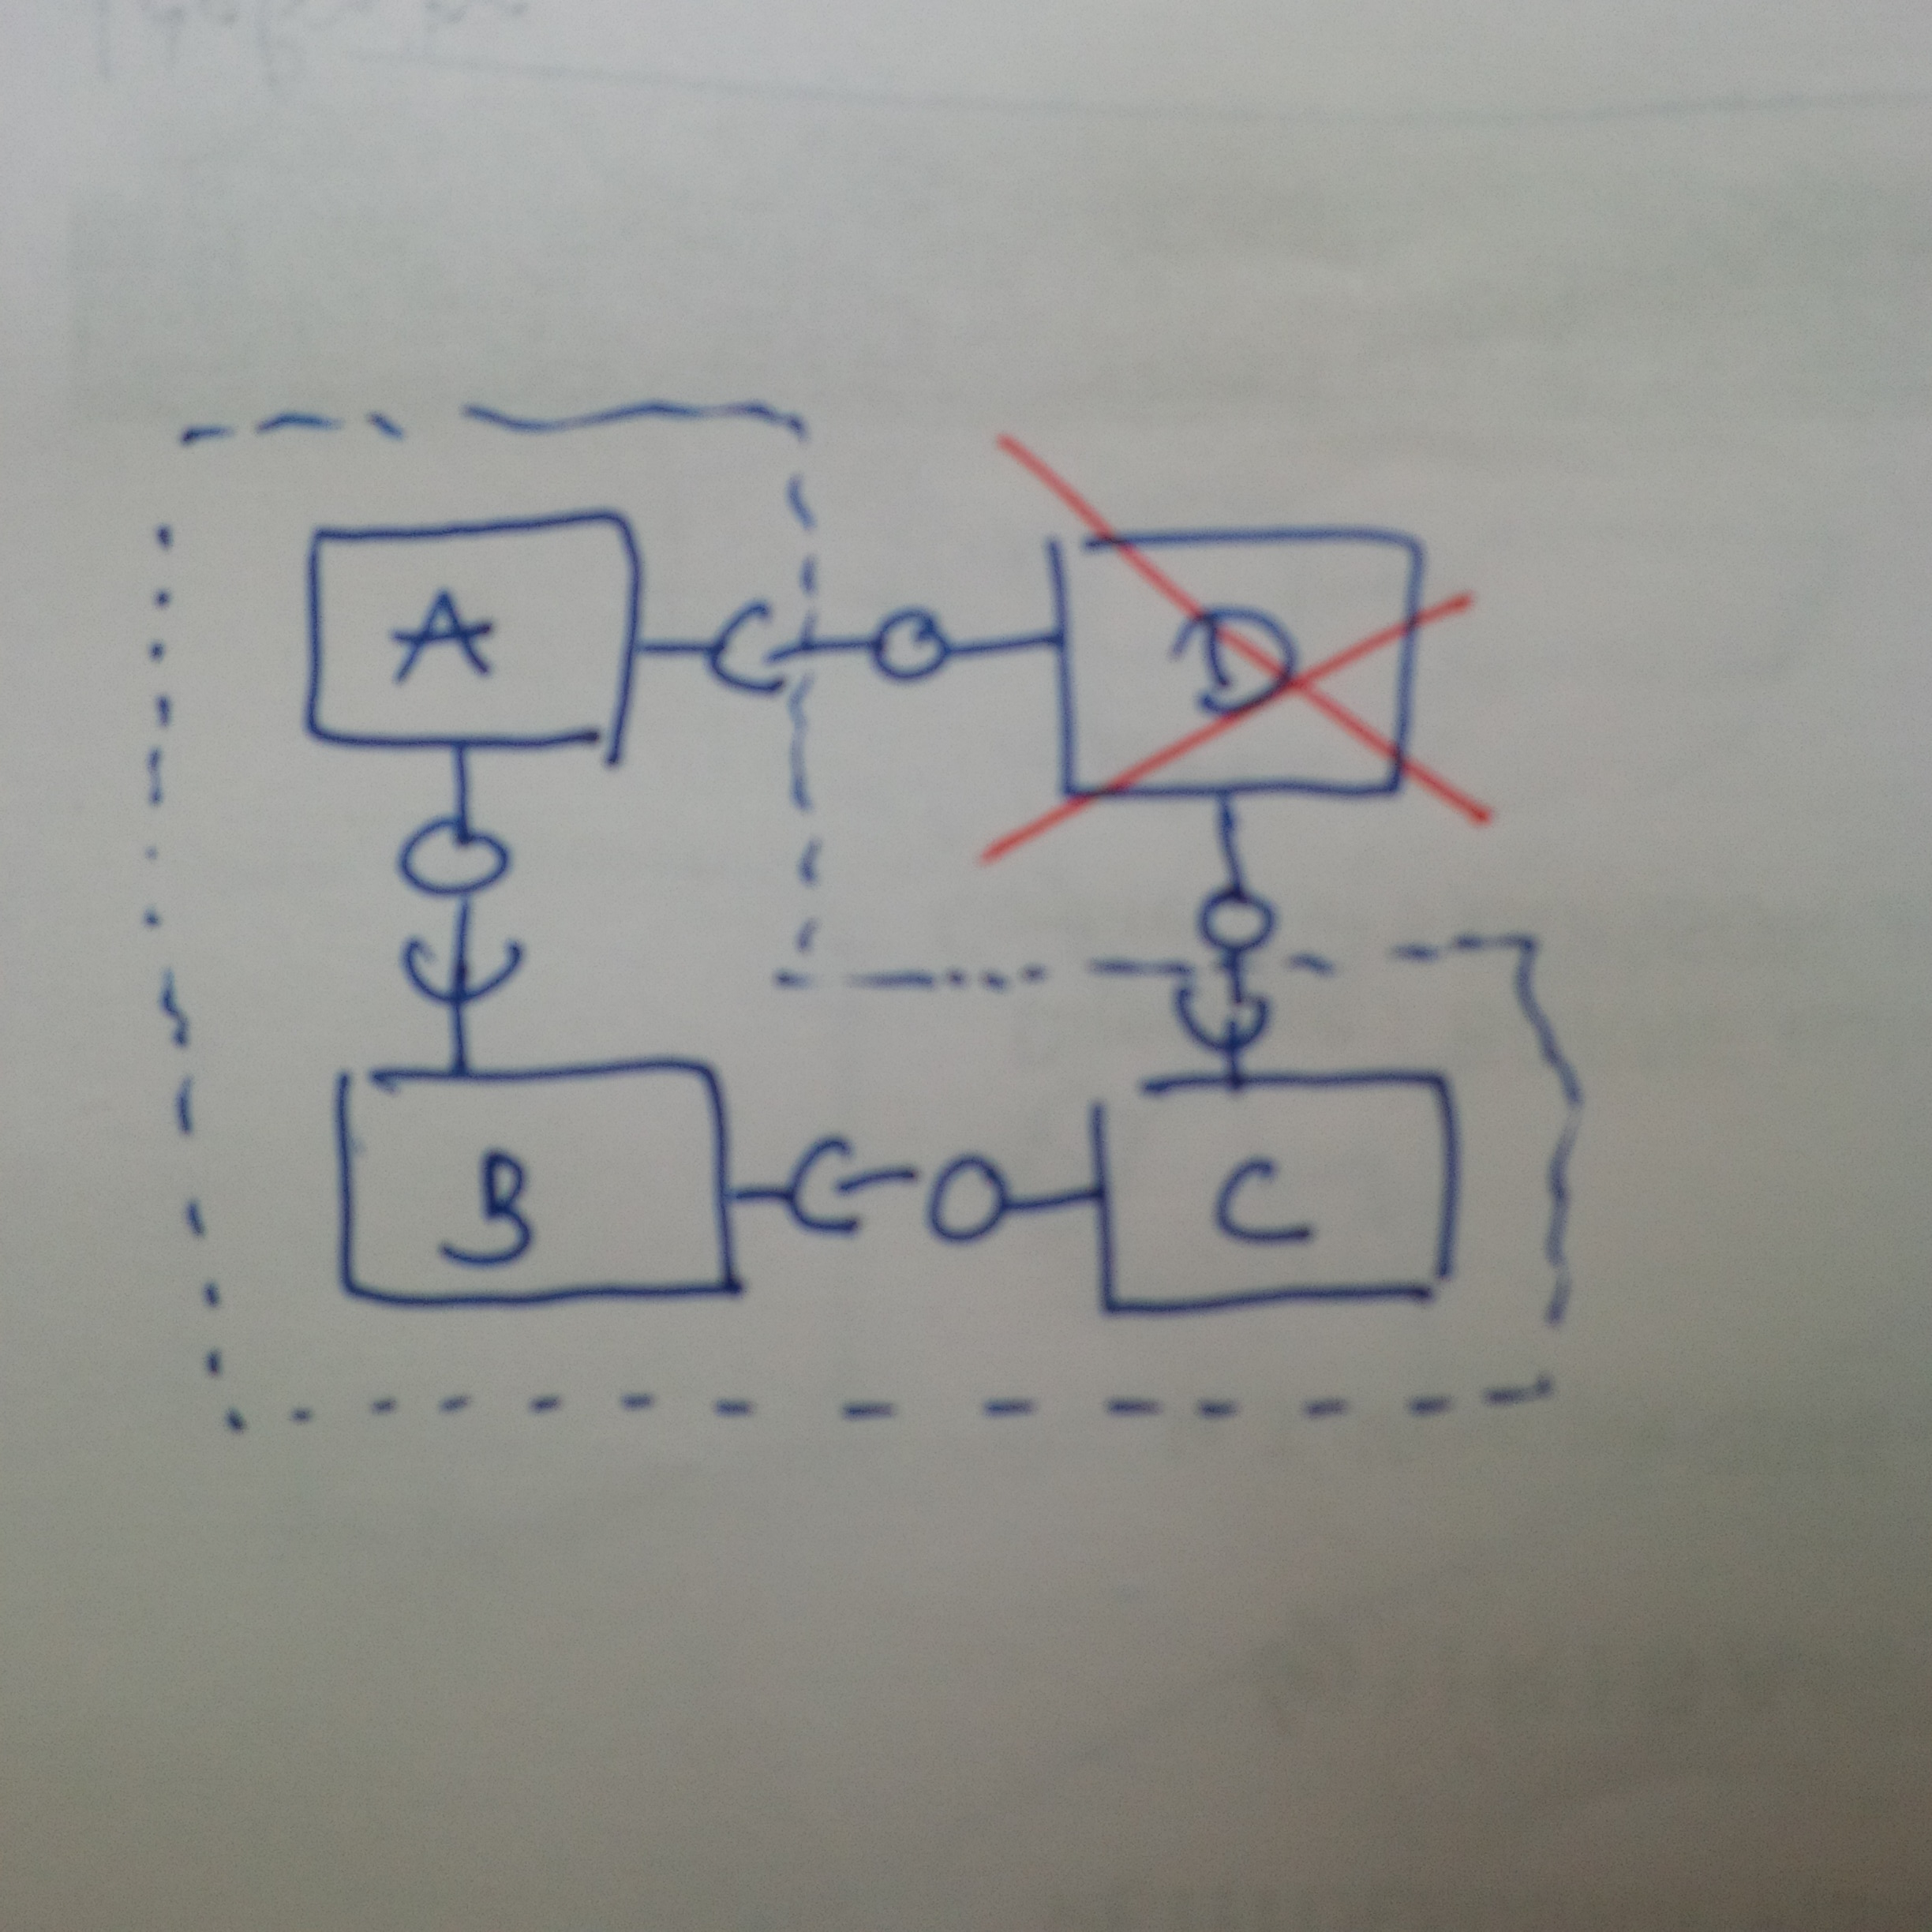
\includegraphics[scale=0.025]{imgs/slide_section1_probleme_frontiere.jpg}
\end{block}

\begin{block}{Approche}
\centering
Étude des langages et processus de modélisation.
\begin{figure} 
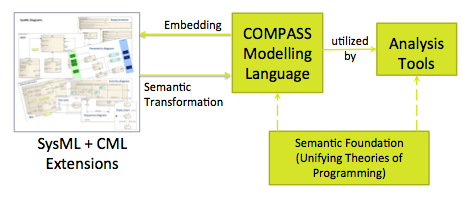
\includegraphics[width=4cm, height=1.5cm]{imgs/compass.png}
\hspace{0.5cm}
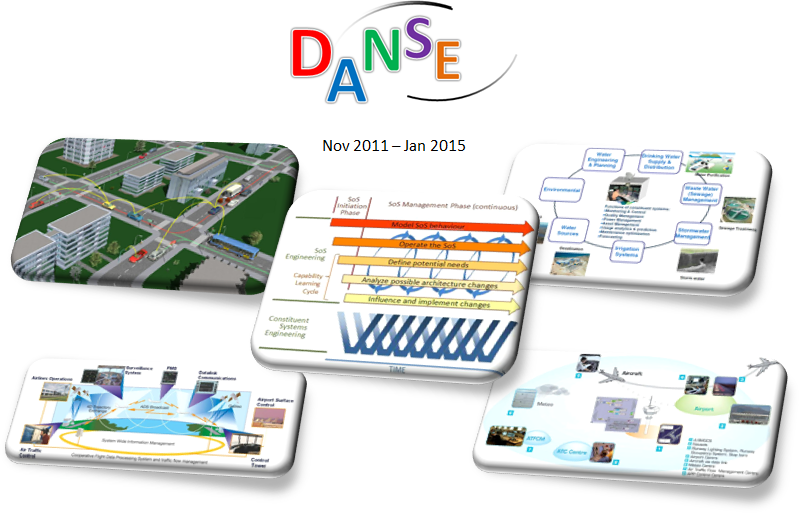
\includegraphics[width=4cm, height=1.5cm]{imgs/danse.png}
\end{figure}
\end{block} 

\end{frame}

\begin{frame}{COMPASS et DANSE : langage, portée et processus}
\end{frame}

%\begin{frame}{Comparaison de DANSE et COMPASS}
%- objectif de modélisation des vues pareil\\
%- utilisation des diagrammes différentes pour modéliser les objetctifs d'interaction\\
%les points négatifs : \\
%- pas de vérification de l'exactide. raffinement des propriétés dans des langages formelles\\
%\end{frame}

\begin{frame}{Stratégie de modélisation}
\end{frame}

